\documentclass{beamer}

\usepackage[utf8]{inputenc}
\usepackage{default}

\mode<presentation>
%{ \usetheme{boxes} }


\usetheme{Madrid}

\usepackage{times}
\usepackage{graphicx}
\usepackage{tabulary}
\usepackage{listings}
\usepackage{verbatimbox}
\usepackage{graphicx}
\usepackage{lmodern}
\usepackage[absolute,overlay]{textpos}
\usepackage{pgfpages}
\usepackage{color}

\pgfdeclareimage[height=1.0cm]{logo_rcc}{icons/logo_rcc.png}
\setlength{\TPHorizModule}{1mm}
\setlength{\TPVertModule}{1mm}
\newcommand{\RCCLogo}{
\begin{textblock}{14}(1.5,1.5)
  \pgfuseimage{logo_rcc}
\end{textblock}
}

\definecolor{mycolorcli}{RGB}{53,154,26}
\definecolor{mycolorcode}{RGB}{0,0,255}
\definecolor{mycolordef}{RGB}{255,0,0}
\definecolor{mycolorlink}{RGB}{184,4,255}

\title{\huge{Introduction to Hadoop}}
\author{Igor Yakushin \\ \texttt{ivy2@uchicago.edu}}
%\date{January 20, 2018}

\definecolor{ChicagoMaroon}{RGB}{128,0,0}

\setbeamercolor{title}{bg=ChicagoMaroon}

\begin{document}

\setbeamertemplate{navigation symbols}{}

\setbeamercolor{fcolor}{fg=white,bg=ChicagoMaroon}
\setbeamertemplate{footline}{
\begin{beamercolorbox}[ht=4ex,leftskip=1.4cm,rightskip=.3cm]{fcolor}
\hrule
\vspace{0.1cm}
   \hfill \insertshortdate \hfill \insertframenumber/\inserttotalframenumber
\end{beamercolorbox}
}

\setbeamercolor{frametitle}{bg=ChicagoMaroon,fg=white}

\begin{frame}
\titlepage
\end{frame}

\section{Login and slides}
\begin{frame}[fragile]
  \frametitle{Login and slides}

  \begin{itemize}
  \item If you do not have an account on Hadoop cluster, use yubikey:
    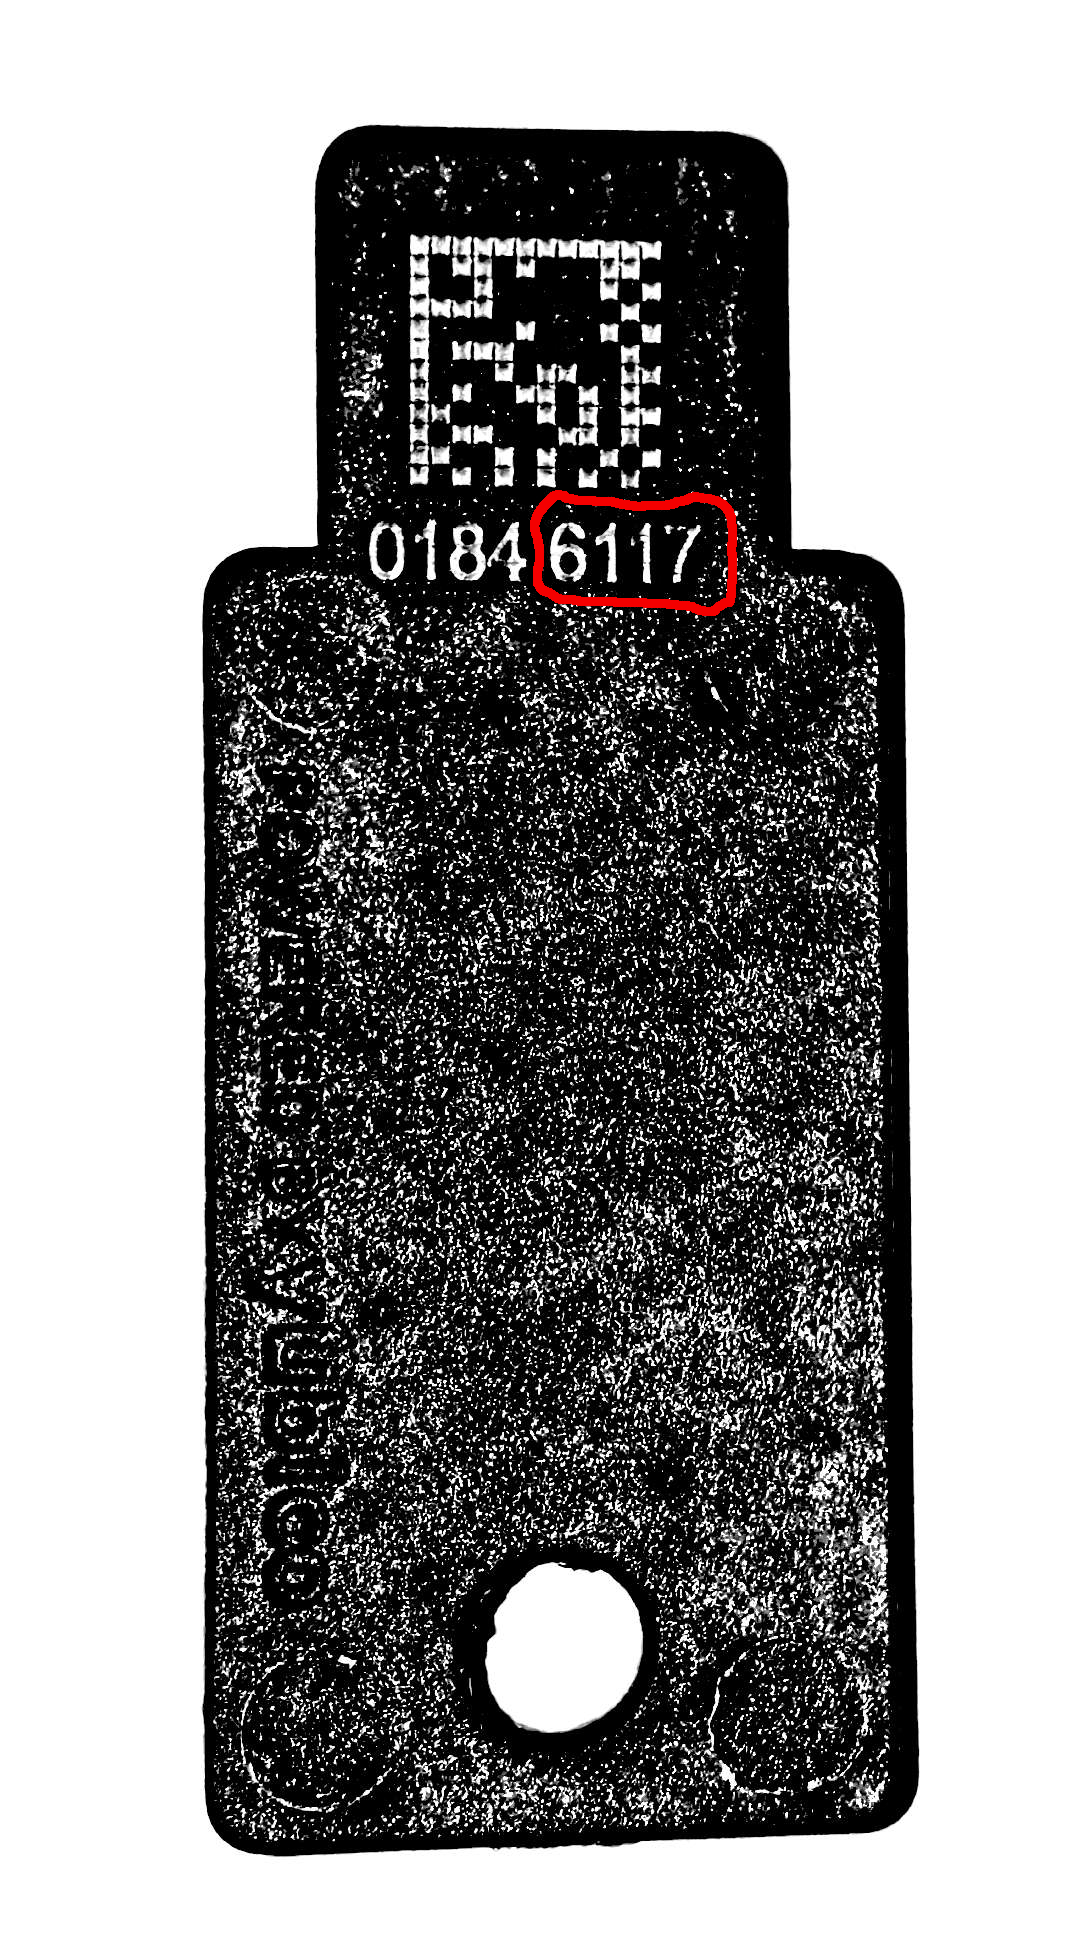
\includegraphics[width=1.5cm]{icons/yubikey1a.jpg}
    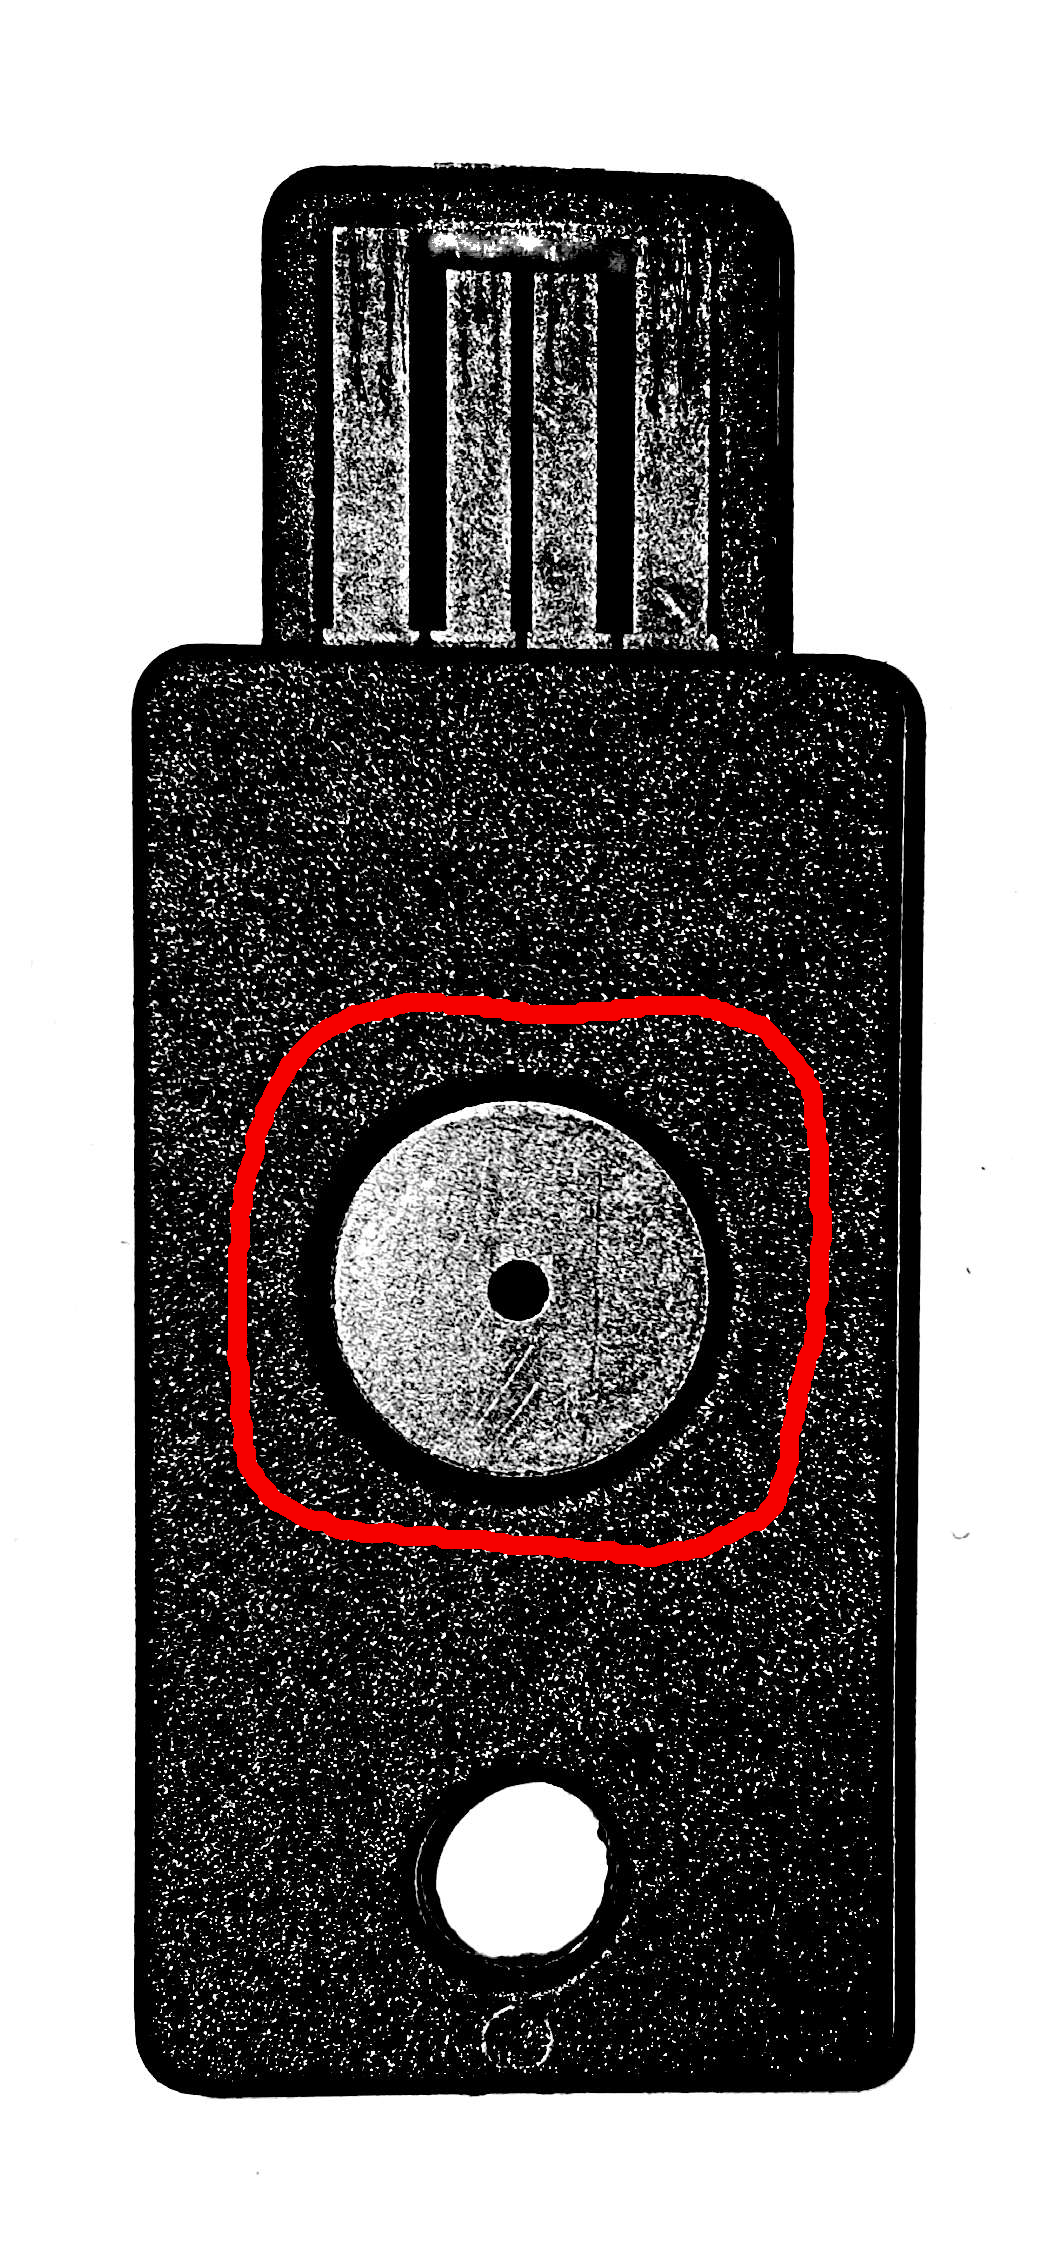
\includegraphics[width=1.3cm]{icons/yubikey2a.jpg}
    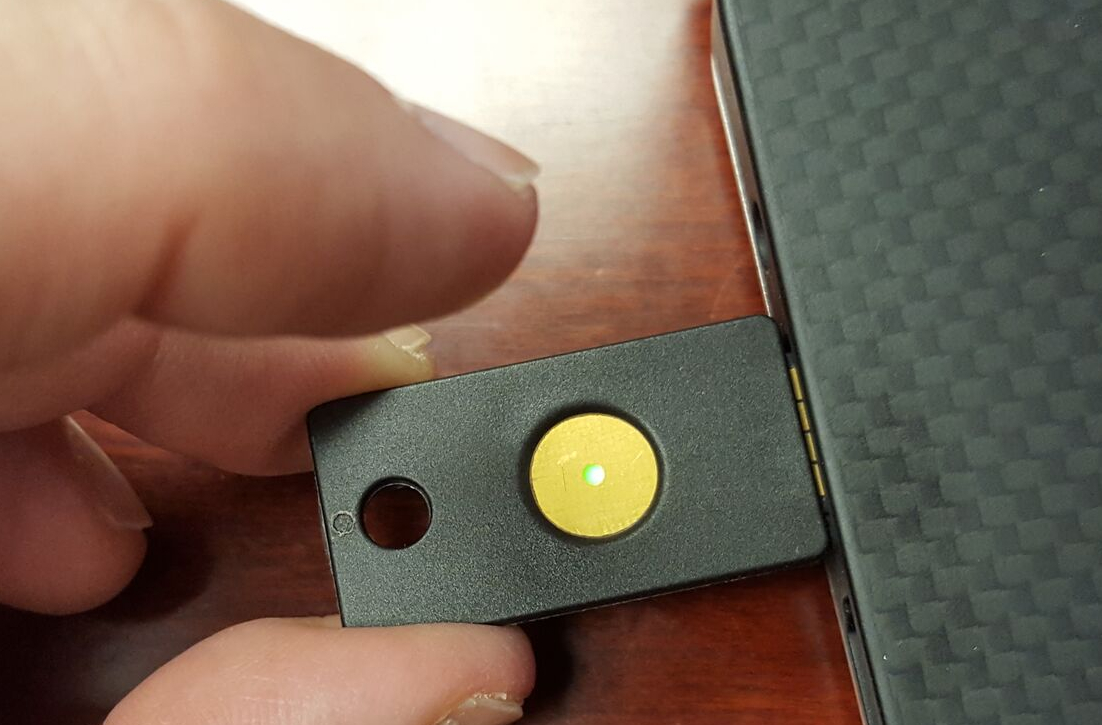
\includegraphics[width=3.3cm]{icons/yubikey3a.jpg}
  \item Use last 4 digits of yubikey as part of userid:
    {\color{mycolorcli}
\begin{verbatim}
ssh -Y rccguest<XXXX>@hadoop.rcc.uchicago.edu
\end{verbatim}
    }
  \item Push the button when asked for password
  \item If you have an account on Hadoop cluster
    {\color{mycolorcli}
\begin{verbatim}
ssh -Y <username>@hadoop.rcc.uchicago.edu
\end{verbatim}
    }
  \item To get slides and labs, point the browser to:
    {\tiny
      {\color{mycolorcli}
\begin{verbatim}
https://git.rcc.uchicago.edu/ivy2/Graham_Introduction_to_Hadoop
\end{verbatim}
      }
    }
  \item After logging into Hadoop cluster, get code and slides:
    {\tiny
      {\color{mycolorcli}
\begin{verbatim}
git clone https://git.rcc.uchicago.edu/ivy2/Graham_Introduction_to_Hadoop.git
\end{verbatim}
      }
    }
  \end{itemize}
\end{frame}

\subsection{2fa}
\begin{frame}[fragile]
  \frametitle{Login and slides: 2fa}
  \begin{itemize}
  \item Since the end of last year, there is an extra extremely annoying security complication: 
    {\color{mycolordef}2-factor authentication}.
  \item You need to follow the instructions on {\color{mycolorcli}\verb|https://cnet.uchicago.edu/2FA/index.htm|} 
    to enroll in 2-factor authentication.
    Another useful related page: {\color{mycolorcli}\verb|https://2fa.rcc.uchicago.edu|}.
  \item You would need to install an application on your phone so that when you try to connect to midway, 
    you get notification on your phone to which you need to respond
  \item If you do not have a phone or travelling abroad, 
    you can get a set of passcodes that you can type instead, each time using the next passcode from the list and periodically
    getting a new list once you use all the numbers from there.
  \end{itemize}
\end{frame}



%\input{hadoop.tex}

\section{What is Hadoop?}
\begin{frame}
  \frametitle{What is Hadoop?}
  \begin{itemize}
   \item A framework to process huge amount of data
   \item Implemented in Java
   \item Runs on a cluster of commodity computers, from a few to a few thousand nodes
   \item Consists of two major components:
    \begin{itemize}
      \item {\color{mycolordef}HDFS} - distributed file system; everything you put there is automatically divided into blocks that are replicated and spread across the cluster;
      \item {\color{mycolordef}MapReduce} - an approach to perform calculations on such data in parallel.
    \end{itemize}
  \end{itemize}
\end{frame}

\begin{frame}
  \frametitle{Hadoop zoo}
  \begin{itemize}
  \item There is a zoo of other Hadoop related tools
    \begin{itemize}
    \item {\color{mycolordef}Hive} - SQL interface to Hadoop built on top of HDFS and MapReduce
    \item {\color{mycolordef}Impala} - another SQL interface to Hadoop, allegedly much faster
    \item {\color{mycolordef}HBase} - noSQL fast distributed database on top of HDFS
    \item {\color{mycolordef}Pig}  -  data processing languague built on top of HDFS and MapReduce
    \item {\color{mycolordef}Spark} - for performance reasons no longer relies on MapReduce,
      can be used without Hadoop; its native language is Scala but it can also be used from Java, Python, R
    \item {\color{mycolordef}Sqoop} - copy data between relational database and Hadoop
    \item {\color{mycolordef}Flume} - copy data into Hadoop, typically used to store logs from a cluster for subsequent analysis
    \item {\color{mycolordef}YARN} - resource allocation manager, used to submit jobs
    \item {\color{mycolordef}Zookeeper} - centralized service for maintaining configuration information, naming, providing distributed synchronization
    \item {\color{mycolordef}Hue} - web GUI to many of the above tools
    \end{itemize}
  \item In Big Data Platform class you'll mostly use pySpark via JupyterHub interface, HDFS, Hive, Pig, Hue.
  \end{itemize}
\end{frame}

\section{Hadoop vs traditional RDBMS}
\subsection{Comparison}
\begin{frame}
  \frametitle{Hadoop vs traditional RDBMS}
  \begin{center}

    \begin{tabulary}{\textwidth}{L | L}
      \hline
      {\color{mycolordef}\textbf{RDBMS}} & {\color{mycolordef}\textbf{Hadoop}} \\ \hline
      do not scale well beyond a few terabytes & easily scales to petabytes by adding more computers to the cluster \\ \hline
      for large datasets runs on very expensive enterprise server & data is scattered on a cluster of cheap commodity computers \\ \hline
      works on structured data; one needs to predefine the data schema & can accept any unstructured data and worry about interpreting and reinterpreting it later \\ \hline
      data needs to be normalized to avoid duplication and enforce constraints & works best on a single denormalized table \\ \hline

    \end{tabulary}

  \end{center}
\end{frame}

\begin{frame}
  \frametitle{Hadoop vs traditional RDBMS}
  \begin{center}

    \begin{tabulary}{\textwidth}{L | L}
      \hline
      {\color{mycolordef}\textbf{RDBMS}} & {\color{mycolordef}\textbf{Hadoop}} \\ \hline
      can be faster for queries on small subset of data & might introduce too much overhead for such queries \\ \hline
      ACID - compliant & in general - not ACID-compliant \\ \hline
      natively speaks SQL & natively implements MapReduce approach in Java on top of which some subset of SQL might be supported \\ \hline 
      is good for banks to keep track of transactions & is good for data scientists to try various ideas on a huge sets of data  \\ \hline
    \end{tabulary}

  \end{center}
\end{frame}

\subsection{ACID compliance}
\begin{frame}
`\frametitle{ACID compliance}
\begin{itemize}
  \item {\color{mycolordef}\textbf{A}}tomicity - The database transaction must completely succeed or completely fail
  \item {\color{mycolordef}\textbf{C}}onsistency - During the database transaction, RDBMS progresses from one valid state to another. The state is never invalid
  \item {\color{mycolordef}\textbf{I}}solation - The client's database transaction must occur in isolation from other clients attempting to transact
  \item {\color{mycolordef}\textbf{D}}urability - Once transaction is committed, it will remain so, 
    even in the event of power loss, crashes, or errors. The data operation that was part of the transaction must be reflected in nonvolatile storage. 
\end{itemize}

Hadoop has no concept of transaction so is not ACID compiliant.

\end{frame}

\section{Distributions}
\begin{frame}
 \frametitle{Distributions}
 There are many Hadoop distributions that bundle different set of tools and add their own:
 \begin{itemize}
  \item {\color{mycolordef}Apache}  - free, open source;
  \item {\color{mycolordef}Cloudera} - we are using Cloudera 6.3;
  \item {\color{mycolordef}Hortonworks} - Hortonworks and Cloudera recently merged but they still maintain two separate distributions and working on the joint one
  \item {\color{mycolordef}HDInsight} - Microsoft  Azure's Cloud based Hadoop Distribution
  \item {\color{mycolordef}MapR}
  \item ...
  \end{itemize}
  Many distributions, for example Cloudera, provide virtual machines to play with
\end{frame}

\section{HDFS}
\subsection{Introduction}
\begin{frame}
 \frametitle{HDFS}
    \begin{itemize}
     \item Any file that is put into HDFS is automatically split into blocks (by default 128M)
     \item Each block is replicated (by default 3 times)
     \item The blocks are spread across the cluster so that
      \begin{itemize}
	\item calculations can be done in parallel on different blocks to increase performance
	\item the file system is fault-taulerant with respect to disk/node/rack failure
	\item if a node goes down, HDFS takes care of creating more replicas automatically
	\item when a node comes back, extra replicas are destroyed
	\item if a new node is added, data spreads on it automatically
	\item there is a {\color{mycolordef}NameNode} that keeps track of where the blocks are
      \end{itemize}
	\item The calculations are done on {\color{mycolordef}DataNodes}
        \item Hadoop tries to do computations where the data is to minimize communication between nodes which is much slower
    \end{itemize} 
\end{frame}

\subsection{Usage}
\begin{frame}[fragile]
  \frametitle{HDFS: user interface}
{\color{mycolorcli}
  \begin{lstlisting}[frame=single, basicstyle=\tiny]
$ hdfs dfs -ls /user/$USER
drwx------   - ivy2 ivy2          0 2016-08-12 20:11 /user/ivy2/.Trash                                                                                                                                                                     

$ hdfs dfs -mkdir /user/$USER/test2 

$ hdfs dfs -put /usr/share/dict/linux.words /user/$USER/test2/

$ hdfs dfs -ls -h  /user/$USER/test2/
-rw-r--r--   3 ivy2 ivy2      4.7 M 2016-08-12 20:12 /user/ivy2/test2/linux.words

$ hdfs dfs -setrep 4  /user/$USER/test2/linux.words
Replication 4 set: /user/ivy2/test2/linux.words

$ hdfs dfs -ls -h  /user/$USER/test2/
-rw-r--r--   4 ivy2 ivy2      4.7 M 2016-08-12 20:12 /user/ivy2/test2/linux.words

$ hdfs dfs -mv /user/$USER/test2/linux.words /user/$USER/test2/words.txt

$ hdfs dfs -get /user/$USER/test2/words.txt

$ hdfs dfs -rm /user/$USER/test2/words.txt
  \end{lstlisting}
}

\begin{itemize}
\item Lab 1
\end{itemize}

\end{frame}


\section{MapReduce}
\subsection{Introduction}
\begin{frame}
 \frametitle{MapReduce}
 \begin{itemize}
  \item {\color{mycolordef}\textbf{map}} - convert each record into $(key, value)$ pairs
  \item {\color{mycolordef}\textbf{reduce}} - apply some reduce operation to the resulting set of $(key, value)$; for example, sum values for each key, or find max, or min, etc.
  \item Obviously, maps can be done in parallel, independently from each other, on different nodes, for each record
  \item Between local map and global reduce, perhaps, apply reduce locally on each node before doing it globally and sort the results
  \item The native way to write your own MapReduce is to extend the corresponding Java classes from MapReduce API
  \item These days people rarely have to implement their own MapReduce but rather use high level tools like Pig, Hive, Spark, HBase, etc. unless you 
    are a programmer implementing such a high level tool
  \end{itemize}
\end{frame}

\subsection{Examples}
\begin{frame}
  \frametitle{Examples of applying MapReduce approach}
  \begin{itemize}
  \item {\color{mycolordef}Count how many times each word occurs in a text}
    \begin{itemize}
      \item map - for each word {\color{mycolorcode}$w_i$} in a record (for example, a line in a text file) output {\color{mycolorcode}$(w_i,1)$}
      \item reduce - for each {\color{mycolorcode}$w_i$} sum the values
    \end{itemize}
  \item {\color{mycolordef}Count the average number of social contacts a person has grouped by age}
    \begin{itemize}
    \item map - for each person {\color{mycolorcode}$p_i$}  of an age {\color{mycolorcode}$a_i$} in a record, output {\color{mycolorcode}$(a_i, (1, contacts_i))$}
    \item reduce - for each age {\color{mycolorcode}$a_i$}, sum separately the first and second component of the value to obtain number 
      of people of a given age and total number of contacts, divide the latter by the former
    \end{itemize}
  \end{itemize}
\end{frame}

\begin{frame}[fragile]
  \frametitle{Examples of applying MapReduce approach}
  \begin{itemize}
  \item {\color{mycolordef}Finding common friends, like in Facebook. } For each person a list of friends is given:
    \begin{lstlisting}[frame=single, basicstyle=\tiny]
      A -> B C D
      B -> A C D E
      C -> A B D E
      D -> A B C E
      E -> B C D
    \end{lstlisting}
    
    \begin{itemize}
    \item map - key is a person and a friend, sorted; value is the list of friends. For example, for C the output from map is:
      \begin{lstlisting}[frame=single, basicstyle=\tiny]
        (A C) -> A B D E
        (B C) -> A B D E
        (C D) -> A B D E
        (C E) -> A B D E
      \end{lstlisting}
    \item reduce - group the results by key, for example:
      \begin{lstlisting}[frame=single, basicstyle=\tiny]
        (A B) -> (A C D E) (B C D)
      \end{lstlisting}
      and find the intersection of value lists:
      \begin{lstlisting}[frame=single, basicstyle=\tiny]
        (A B) -> (C D)
      \end{lstlisting}
    \end{itemize}
  \end{itemize}
\end{frame}


\subsection{Java API}
\begin{frame}[fragile]
 \frametitle{MapReduce: using Java API}

\begin{itemize}
\item Import various Hadoop related modules:
\end{itemize}
{\color{mycolorcode}
  \begin{lstlisting}[frame=single, basicstyle=\tiny,language=java]
import java.io.IOException;
import java.util.StringTokenizer;

import org.apache.hadoop.conf.Configuration;
import org.apache.hadoop.fs.Path;
import org.apache.hadoop.io.IntWritable;
import org.apache.hadoop.io.Text;
import org.apache.hadoop.mapreduce.Job;
import org.apache.hadoop.mapreduce.Mapper;
import org.apache.hadoop.mapreduce.Reducer;
import org.apache.hadoop.mapreduce.lib.input.FileInputFormat;
import org.apache.hadoop.mapreduce.lib.output.FileOutputFormat;
  \end{lstlisting}
}
\end{frame}


\begin{frame}[fragile]
 \frametitle{MapReduce: using Java API}

\begin{itemize}
  \item Inside your own {\color{mycolorcode}WordCount} class, create a class that extends {\color{mycolorcode}Mapper}:
\end{itemize}
{\color{mycolorcode}
  \begin{lstlisting}[frame=single, basicstyle=\tiny,language=java]
public class WordCount {

  public static class TokenizerMapper
      extends Mapper<Object, Text, Text, IntWritable>{

      private final static IntWritable one = new IntWritable(1);
      private Text word = new Text();

      public void map(Object key, Text value, Context context
                      ) throws IOException, InterruptedException {
          StringTokenizer itr = new StringTokenizer(value.toString());
          while (itr.hasMoreTokens()) {
              word.set(itr.nextToken());
              context.write(word, one);
          }
      }
  }
}
  \end{lstlisting}
}
\begin{itemize}
  \item {\color{mycolorcode}TokenizerMapper} overwrites {\color{mycolorcode}map} method to split each line into words and return {\color{mycolorcode}$(word, 1)$} for each {\color{mycolorcode}$word$}.
\end{itemize}

\end{frame}


\begin{frame}[fragile]
 \frametitle{MapReduce: using Java API}
\begin{itemize}
  \item {\color{mycolorcode}IntSumReducer} extends {\color{mycolorcode}Reducer} class and overwrites its {\color{mycolorcode}reduce} method to count number of words:
\end{itemize}
{\color{mycolorcode}
  \begin{lstlisting}[frame=single, basicstyle=\tiny,language=java]
  public static class IntSumReducer
      extends Reducer<Text,IntWritable,Text,IntWritable> {
      private IntWritable result = new IntWritable();

      public void reduce(Text key, Iterable<IntWritable> values,
                       Context context
                         ) throws IOException, InterruptedException {
          int sum = 0;
          for (IntWritable val : values) {
              sum += val.get();
          }
          result.set(sum);
          context.write(key, result);
      }
  }
  \end{lstlisting}
}
\end{frame}


\begin{frame}[fragile]
 \frametitle{MapReduce: using Java API}

\begin{itemize}
  \item {\color{blue}main} function sets up configuration, launches MapReduce job and writes the results to a file:
\end{itemize}
{\color{mycolorcode}
  \begin{lstlisting}[frame=single, basicstyle=\tiny,language=java]
    public static void main(String[] args) throws Exception {
        Configuration conf = new Configuration();
        Job job = Job.getInstance(conf, "word count");
        job.setJarByClass(WordCount.class);
        job.setMapperClass(TokenizerMapper.class);
        job.setCombinerClass(IntSumReducer.class);
        job.setReducerClass(IntSumReducer.class);
        job.setOutputKeyClass(Text.class);
        job.setOutputValueClass(IntWritable.class);
        FileInputFormat.addInputPath(job, new Path(args[0]));
        FileOutputFormat.setOutputPath(job, new Path(args[1]));
        System.exit(job.waitForCompletion(true) ? 0 : 1);
    }
}
  \end{lstlisting}
}
\end{frame}

\begin{frame}[fragile]
 \frametitle{MapReduce: using Java API}
{\color{mycolorcli}
  \begin{lstlisting}[frame=single, basicstyle=\tiny]
source env.sh
mkdir wordcount_classes
javac -cp /opt/cloudera/parcels/CDH/lib/hadoop/*:\
          /opt/cloudera/parcels/CDH/lib/hadoop/client-0.20/*\ 
          -d wordcount_classes WordCount.java
jar -cvf wordcount.jar -C wordcount_classes/ .

hdfs dfs -mkdir /user/$USER/wordcount
hdfs dfs -rm -r -f /user/$USER/wordcount/output
hdfs dfs -put  /software/matlab-2014b-x86_64/\
               toolbox/distcomp/examples/integration/old/pbs/README 
               /user/$USER/wordcount/

hadoop jar wordcount.jar WordCount 
           /user/$USER/wordcount/README /user/$USER/wordcount/output

hdfs dfs -ls /user/ivy2/wordcount/output
hdfs dfs -cat wordcount/output/part-r-00000
hdfs dfs -cat wordcount/output/part-r-000* | sort > out.txt
hdfs dfs -getmerge wordcount/output merged.txt
cat merged.txt | grep sort
\end{lstlisting}
}

\begin{itemize}
\item Lab 2
\end{itemize}

\end{frame}

  
\subsection{Streaming}
  \begin{frame}[fragile]
 \frametitle{MapReduce: using streaming}
 \begin{itemize}
 \item Streaming interface allows one to write MapReduce in any language although the functionality is limited and the performance is worse than what one can
 get by using native Java API. 
\item Mapper takes input from stdin, breaks it into records - lines in a text file - and is expected to print to stdout pairs of key and value separated by Tab;
  everything before the first Tab is considered a key, the rest of the line is considered a value
 \item Similarly reducer is expected to receive such pairs in stdin and prints its results to stdout
 \item When launching a job, one needs to use Hadoop's streaming jar and specify mapper, reducer, input and output files as options

 \end{itemize}
\end{frame}

  
\begin{frame}[fragile]
 \frametitle{MapReduce: using streaming}

 \begin{itemize}
   \item In this example we implement {\color{mycolorcli}WordCount.java} functionality in python
   \item {\color{mycolorcli}mapper.py}:
{\color{mycolorcode}
  \begin{lstlisting}[frame=single, basicstyle=\tiny,language=python]
import sys

for line in sys.stdin:
    line = line.strip()
    words = line.split()
    for word in words:
        print '%s\t%s' % (word, 1)

 \end{lstlisting} 
}
 \end{itemize}

\end{frame}

\begin{frame}[fragile]
 \frametitle{MapReduce: using streaming}
\begin{itemize}
  \item {\color{mycolorcli}reducer.py}:
{\color{mycolorcode}
  \begin{lstlisting}[frame=single, basicstyle=\tiny,language=python]
from operator import itemgetter
import sys

current_word = None
current_count = 0
word = None

for line in sys.stdin: 
    line = line.strip()
    word, count = line.split('\t', 1)
    try:
        count = int(count)
    except ValueError:
        continue

    if current_word == word:
        current_count += count
    else:
        if current_word:
            print '%s\t%s' % (current_word, current_count)
        current_count = count
        current_word = word

if current_word == word:
    print '%s\t%s' % (current_word, current_count)
 \end{lstlisting}
}
\end{itemize}
\end{frame}

\begin{frame}[fragile]
 \frametitle{MapReduce: using streaming}

 \begin{itemize}
   \item To run a job:
{\color{mycolorcli}
  \begin{lstlisting}[frame=single, basicstyle=\tiny]
hadoop jar /opt/cloudera/parcels/CDH/lib/hadoop-mapreduce/hadoop-streaming.jar \ 
       -input /user/$USER/wordcount/README \
       -output /user/$USER/wordcount/streaming-out-py \ 
       -file mapper.py -mapper mapper.py -file reducer.py -reducer reducer.py
 \end{lstlisting}
}

\item Lab 3

 \end{itemize}


\end{frame}

\section{HBase}
\subsection{Introduction}
\begin{frame}
  \frametitle{HBase}
  \begin{itemize}
  \item {\color{mycolordef}\textbf{H}}adoop data{\color{mycolordef}\textbf{Base}}
  \item Consists of tables
  \item Each table is sparse, distributed, persistent, multidimensional sorted map, indexed by rowkey, column family, column, timestamp
  \item Can store structured, semistructured, unstructured data
  \item Does not care about types
  \item Not a relational database, does not speak SQL natively, does not enforce relationship in data
  \item Designed to run on a cluster of computers, scale horizontally as you add more machines to the cluster
  \item The main operations are: create (table), put (value into cell), get (value from cell), scan (values from cells)
  \item Various auxiliary operations: alter, list, describe, ...
  \end{itemize}
\end{frame}

\begin{frame}[fragile]
 \frametitle{HBase}
 {\color{mycolorcode}
 \begin{verbnobox}[\tiny]
  Row Key     Column Family: {Column Qualifier:Version:Value}
  ------------------------------------------------------------------------
  00001       CustomerName:  {‘FN’: 1383859182496:‘John’,
                             ‘LN’: 1383859182858:‘Smith’,
                             ‘MN’: 1383859183001:’Timothy’,
                             ‘MN’: 1383859182915:’T’}
              ContactInfo:   {‘EA’: 1383859183030:‘John.Smith@xyz.com’,
                            ’SA’: 1383859183073:’1 Hadoop Lane, NY 11111’}
  00002       CustomerName:  {‘FN’: 1383859183103:‘Jane’,
                             ‘LN’: 1383859183163:‘Doe’,
              ContactInfo:   {’SA’: 1383859185577:’7 HBase Ave, CA 22222’}
 \end{verbnobox}
 }
 \begin{itemize}
 \item Internally HBase table is stored in {\color{mycolordef}HFiles} - different set of files for different column families
 \item HFiles for the same column family are periodically merged together or split and distributed among the nodes to maintain high performance and fault-taulerance
 \item On top of HDFS
 \item One can specify how many latest versions of data to keep in HBase table or to query versions in a particular date-time range
\end{itemize}
\end{frame}

\subsection{Usage: shell}
\begin{frame}[fragile]
 \frametitle{HBase: shell, create, put, list, describe}
{\color{mycolorcli}
  \begin{lstlisting}[frame=single, basicstyle=\tiny]
$ hbase shell

> create 'CustomerContactInfo', 'CustomerName', 'ContactInfo'
> put 'CustomerContactInfo', '00001', 'CustomerName:FN', 'John'
> put 'CustomerContactInfo', '00001', 'CustomerName:LN', 'Smith'
> put 'CustomerContactInfo', '00001', 'CustomerName:MN', 'T'
> put 'CustomerContactInfo', '00001', 'ContactInfo:EA', 'John.Smith@xyz.com'
> put 'CustomerContactInfo', '00001', 'ContactInfo:SA', '1 Hadoop Lane, NY 11111'
> put 'CustomerContactInfo', '00002', 'CustomerName:FN', 'Jane'
> put 'CustomerContactInfo', '00002', 'CustomerName:LN', 'Doe'
> put 'CustomerContactInfo', '00002', 'ContactInfo:SA', '7 HBase Ave, CA 22222'
>list
=> ["CustomerContactInfo"]
>describe 'CustomerContactInfo'
Table CustomerContactInfo is ENABLED
CustomerContactInfo
COLUMN FAMILIES DESCRIPTION                                     
{NAME => 'ContactInfo', DATA_BLOCK_ENCODING => 'NONE', BLOOMFILTER => 'ROW', 
REPLICATION_SCOPE => '0', VERSIONS => '1', COMPRESSION => 'NONE', 
MIN_VERSIONS => '0', TTL => 'FOREVER', KEEP_DELETED_CELLS => 'FALSE', 
BLOCKSIZE => '65536', IN_MEMORY => 'false', BLOCKCACHE => 'true'}           
{NAME => 'CustomerName', DATA_BLOCK_ENCODING => 'NONE', BLOOMFILTER => 'ROW', 
REPLICATION_SCOPE => '0', VERSIONS => '1', COMPRESSION => 'NONE', MIN_VERSIONS => '0', 
TTL => 'FOREVER', KEEP_DELETED_CELLS => 'FALSE', BLOCKSIZE => '65536', 
IN_MEMORY => 'false', BLOCKCACHE => 'true'}                                     
  \end{lstlisting}
}
\end{frame}

\begin{frame}[fragile]
 \frametitle{HBase: alter, scan, VERSIONS}
{\color{mycolorcli}
  \begin{lstlisting}[frame=single, basicstyle=\tiny]

> alter 'CustomerContactInfo', NAME => 'CustomerName', VERSIONS => 5
> describe 'CustomerContactInfo'
Table CustomerContactInfo is ENABLED                                     
CustomerContactInfo
COLUMN FAMILIES DESCRIPTION
{NAME => 'ContactInfo', DATA_BLOCK_ENCODING => 'NONE', BLOOMFILTER => 'ROW', 
REPLICATION_SCOPE => '0', VERSIONS => '1', COMPRESSION => 'NONE', 
MIN_VERSIONS => '0', TTL => 'FOREVER', KEEP_DELETED_CELLS => 'FALSE', 
BLOCKSIZE => '65536', IN_MEMORY => 'false', BLOCKCACHE => 'true'}                                     
{NAME => 'CustomerName', DATA_BLOCK_ENCODING => 'NONE', BLOOMFILTER => 'ROW', 
REPLICATION_SCOPE => '0', VERSIONS => '5', COMPRESSION => 'NONE', 
MIN_VERSIONS => '0', TTL => 'FOREVER', KEEP_DELETED_CELLS => 'FALSE', 
BLOCKSIZE => '65536', IN_MEMORY => 'false', BLOCKCACHE => 'true'}
> put 'CustomerContactInfo', '00001', 'CustomerName:MN', 'Timothy'
> scan 'CustomerContactInfo', {VERSIONS => 2}
ROW      COLUMN+CELL 
00001    column=ContactInfo:EA, timestamp=1471196578957, value=John.Smith@xyz.com 
00001    column=ContactInfo:SA, timestamp=1471196578988, value=1 Hadoop Lane, NY 11111 
00001    column=CustomerName:FN, timestamp=1471196578805, value=John 
00001    column=CustomerName:LN, timestamp=1471196578859, value=Smith 
00001    column=CustomerName:MN, timestamp=1471197270641, value=Timothy 
00001    column=CustomerName:MN, timestamp=1471196578901, value=T 
00002    column=ContactInfo:SA, timestamp=1471196579070, value=7 HBase Ave, CA 22222 
00002    column=CustomerName:FN, timestamp=1471196579016, value=Jane 
00002    column=CustomerName:LN, timestamp=1471196579042, value=Doe
  \end{lstlisting}
}
\end{frame}

\begin{frame}[fragile]
 \frametitle{HBase: get, disable, drop, quit}
{\color{mycolorcli}
  \begin{lstlisting}[frame=single, basicstyle=\tiny]
> get 'CustomerContactInfo', '00001'
COLUMN                CELL 
ContactInfo:EA        timestamp=1471196578957, value=John.Smith@xyz.com 
ContactInfo:SA        timestamp=1471196578988, value=1 Hadoop Lane, NY 11111 
CustomerName:FN       timestamp=1471196578805, value=John 
CustomerName:LN       timestamp=1471196578859, value=Smith 
CustomerName:MN       timestamp=1471197270641, value=Timothy
> get 'CustomerContactInfo', '00001', {COLUMN => 'CustomerName:MN'}
COLUMN                CELL 
CustomerName:MN       timestamp=1471197270641, value=Timothy
> disable 'CustomerContactInfo'
> drop 'CustomerContactInfo'
> quit
  \end{lstlisting}
}
\begin{itemize}
\item Lab 4
\end{itemize}
\end{frame}


\subsection{Other clients}
\begin{frame}
 \frametitle{HBase: clients}
 Besides hbase shell, one can use HBase with
 \begin{itemize}
  \item MapReduce
  \item Hive
  \item Pig
  \item Spark
  \item Impala
  \end{itemize}
\end{frame}


\section{Pig}
\subsection{Introduction}
\begin{frame}[fragile]
 \frametitle{Pig: introduction}
 \begin{itemize}
  \item High level language - {\color{mycolordef}\textbf{Pig Latin}}
  \item Compiler translates Pig Latin into MapReduce jobs
  \item It is a {\color{mycolordef}\textbf{dataflow language}} where you define a data stream and a set of transformations applied to it.
  \item Operations: load, store, dump, filter, foreach, group, join, order by, distinct, limit, sample, etc.
  \item You can specify data types to help Pig to optimize a program or you can let it figure it out
 \end{itemize}
\end{frame}


\subsection{How to run}
\begin{frame}[fragile]
 \frametitle{Pig: how to run}
 Pig programs can run in three ways: 
 \begin{itemize}
   \item as a script
     \begin{itemize} 
     \item on a local computer
{\color{mycolorcli}
       \begin{lstlisting}[frame=no, basicstyle=\tiny]
         pig -x local milesPerCarrier.pig
       \end{lstlisting}
}
     \item on a cluster
{\color{mycolorcli}
       \begin{lstlisting}[frame=no, basicstyle=\tiny]
         pig -x mapreduce milesPerCarrier.pig
       \end{lstlisting}
}       
     \end{itemize}
   \item interactively using Grunt interpreter
{\color{mycolorcli}
       \begin{lstlisting}[frame=no, basicstyle=\tiny]
         pig -x local
       \end{lstlisting}
}            
   \item Embedded in other languages such as Java, Python, JavaScript
 \end{itemize}
\end{frame}


\subsection{Examples}
\begin{frame}[fragile]
 \frametitle{Pig: examples}
{\color{mycolorcode}
  \begin{lstlisting}[frame=single, basicstyle=\tiny]
records = LOAD 'pig/words.csv' USING PigStorage(',') AS (W, N:int);
mrecs = GROUP records ALL;
tot = FOREACH mrecs GENERATE SUM(records.N);
DUMP tot;
  \end{lstlisting}

  \begin{lstlisting}[frame=single, basicstyle=\tiny]
in = load 'pig/mary.txt' as (line);
-- TOKENIZE splits the line into a field for each word.
-- flatten will take the collection of records returned by
-- TOKENIZE and produce a separate record for each one, calling the single
-- field in the record word.
words = foreach in generate flatten(TOKENIZE(line)) as word;
grpd = group words by word;
cntd = foreach grpd generate group, COUNT(words);
store cntd into 'cntd.out';
  \end{lstlisting}

  \begin{lstlisting}[frame=single, basicstyle=\tiny]
records = LOAD 'words.csv' USING PigStorage(',') AS (W, N:int);
r1 = filter records by N < 10;
dump r1;
r2 = foreach r1 generate N*N as N2, W;
describe r2;
r3 = join r1 by W, r2 by W;
  \end{lstlisting}
}

\begin{itemize}
\item Lab 5
\end{itemize}

\end{frame}


\section{Hive}
\subsection{Introduction}
\begin{frame}
 \frametitle{Hive: introduction}
 \begin{itemize}
  \item Hive provides Hadoop with SQL access to data
  \item Hive server, sitting on top of HDFS and MapReduce, accepts connections from various Hive clients via, for example, ODBC, JDBC drivers and converts SQL into MapReduce jobs
  \item Hive supports a large subset of SQL including joins
  \item One can create indexes to improve performance
  \item When creating a table, one specifies where the data is stored: textfile, HBase table or any other of numerous data formats supported by Hadoop and residing on HDFS
 \end{itemize}

\end{frame}

\subsection{Example}
\begin{frame}[fragile]
  \frametitle{Hive: example}
{\color{mycolorcode}
  \begin{lstlisting}[frame=single, basicstyle=\tiny]
$ hive
hive> set hive.cli.print.current.db=true;
hive> CREATE DATABASE my1;
hive> USE my1;
hive (my1)> CREATE TABLE t1(W STRING, N INT) ROW FORMAT DELIMITED FIELDS TERMINATED BY ',';
hive (my1)> LOAD DATA INPATH 'words.csv' INTO TABLE t1;
hive (my1)> select count(*) from t1;
hive (my1)> select max(N) from t1;
\end{lstlisting}
}
\begin{itemize}
\item To avoid collision, everybody should use a separate database named by username
\item Interactive usage is only good for experimentation, don't use it for homework. Instead, prepare
  a sql script, for example, {\color{mycolorcli}\verb|my.sql|}, and execute it as follows:
{\color{mycolorcli}
\begin{verbatim}
hive -f my.sql > out.txt 2> err.txt
\end{verbatim}
}
and submit three files as homework: {\color{mycolorcli}\verb|my.sql|}, {\color{mycolorcli}\verb|out.txt|} and 
{\color{mycolorcli}\verb|err.txt|}.
\item You can also run sql on hive database as follows:
{\color{mycolorcli}
\begin{verbatim}
hive --database my1 -e 'select count(*) from t1;'
\end{verbatim}
}
\item Lab 6
\end{itemize}

\end{frame}


\section{Sqoop}
\subsection{Introduction}
\begin{frame}
 \frametitle{Sqoop: introduction}
 
  \begin{itemize}
    \item Sqoop is used to import/export data from/to relational database
    \item In the process of importing one can execute SQL to downselect or denormalize data
    \item Can import into HBase, Hive or HDFS
    \item Can export from HDFS only
    \item Uses JDBC driver to connect to databases
  \end{itemize} 
\end{frame}

\subsection{Examples}
\begin{frame}[fragile]
 \frametitle{Sqoop: examples}
{\color{mycolorcli}
  \begin{lstlisting}[frame=single, basicstyle=\tiny]
$ sqoop import \
--connect jdbc:mysql://localhost/serviceorderdb \
--username root -P \
--table serviceorders -m 1 \
--class-name serviceorders \
--target-dir /usr/biadmin/serviceorders-import \
--bindir .
Enter password:
\end{lstlisting}

\begin{lstlisting}[frame=single, basicstyle=\tiny]
$ sqoop import --connect jdbc:mysql://localhost/serviceorderdb \
--username root -P -m 2 \
--query 'SELECT customercontactinfo.customername, customercontactinfo.
contactinfo FROM customercontactinfo JOIN
serviceorders ON customercontactinfo.customernum = serviceorders.customernum
WHERE $CONDITIONS' \
--split-by serviceorders.serviceordernum \
--boundary-query "SELECT min(serviceorders.serviceordernum),
max(serviceorders.serviceordernum) FROM serviceorders" \
--target-dir /usr/biadmin/customers \
--verbose
\end{lstlisting}

}

\end{frame}

\section{Flume}
\begin{frame}
 \frametitle{Flume}
 \begin{itemize}
  \item Apache Flume is used to propagate data from various sources into Hadoop.
  \item A typical example is to use Flume to collect logs from a cluster
  \item Flume agent
    \begin{itemize}
      \item runs on each node
      \item can accept multiple input channels, transform data and send it to multiple output sinks, local or remote;
    \end{itemize}
 \end{itemize}

 \begin{figure}[h]
 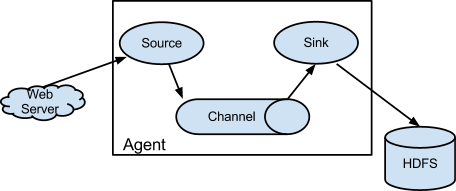
\includegraphics[width=6cm]{graphs/DevGuide_image00.png}
 \end{figure}
 
\end{frame}


\begin{frame}[fragile]
 \frametitle{Flume}
 \begin{itemize}
  \item Flume agents can be connected in a tree: data is collected from all the nodes in a cluster and inserted into Hadoop or Solr or file.
 \end{itemize}

 \begin{figure}[h]
 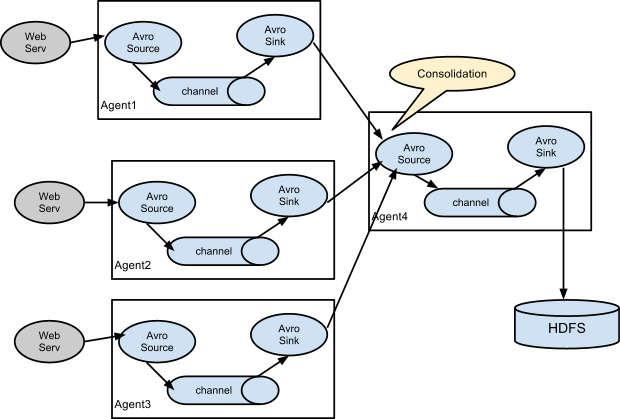
\includegraphics[width=8cm]{graphs/UserGuide_image02.png}
 \end{figure}
\end{frame}

\section{Spark}
\begin{frame}
 \frametitle{Spark}
 \begin{itemize}
  \item Apache Spark - fast general-purpose cluster computing system
  \item API in Scala, Java, Python, R
  \item Rich set of higher-level tools:
    \begin{itemize}
      \item Spark SQL - introduces frames format that is like distributed table; to query data in frames, one can either use Spark or SQL syntax
      \item MLib - library for machine learning
      \item GraphX - library for graph processing
      \item Spark Streaming - scalable, high-throughput stream processing of live data streams.
    \end{itemize}
  \item Spark can be used in combination with BigDL library from Intel that provides deep learning framework
  \item Spark can be used interactively or in batch
  \item It works in Hadoop cluster, in general purpose cluster like midway, on your laptop
  \item It understands Hadoop data formats, can work with HDFS if it is running under Hadoop
 \end{itemize}
\end{frame}

\subsection{RDD}
\begin{frame}
 \frametitle{Spark: RDD}
 \begin{itemize}
  \item Spark's primary abstraction - {\color{mycolordef}\textbf{Resilient Distributed Dataset (RDD)}}
  \item RDD - collection of records partitioned across the nodes and can be operated on in parallel
  \item RDD can be created from HDFS files in various supported formats or by transforming other RDDs
  \item One can ask Spark to {\color{mycolordef}cache RDD in memory or disk} for fast reuse
  \item RDDs automatically recover from node failure
  \item RDD supports two types of operations:
    \begin{itemize}
      \item {\color{mycolordef}\textbf{Transformations}} - create a new dataset from an existing one. Lazy evaluation - evaluated only when required by action.
      \item {\color{mycolordef}\textbf{Actions}} - return a value to the driver program after running a computation on the dataset.
    \end{itemize}
 \end{itemize}
\end{frame}

\subsubsection{Transformations}
\begin{frame}
  \frametitle{Spark: RDD: transformations}
  Examples of RDD transformations:
  \begin{itemize}
  \item {\color{mycolorcode}map(func)} - transform each element by a applying a function
  \item {\color{mycolorcode}filter(func)} - select records satisfying boolean function
  \item {\color{mycolorcode}sample(withReplacement, fraction, seed)} - Sample a fraction fraction of the data, with or without replacement, using a given random number generator seed.
  \item {\color{mycolorcode}union(otherDataset), intersection(otherDataset)}
  \item {\color{mycolorcode}distinct([numTasks]))}
  \item {\color{mycolorcode}groupByKey([numTasks])}
  \item {\color{mycolorcode}sortByKey([ascending], [numTasks])}
  \end{itemize}
\end{frame}

\subsubsection{Actions}
\begin{frame}
  \frametitle{Spark: RDD: actions}
  \begin{itemize}

  \item {\color{mycolorcode}collect()} - Return all the elements of the dataset as an array to the login node. Don't run it until you reduce the data enough on the cluster, it might not fit
    into the memory of the login node.
  \item {\color{mycolorcode}count()}
  \item {\color{mycolorcode}take(n)} - Return first n elements of the results
  \item {\color{mycolorcode}reduce(func)} - Aggregate the elements of the dataset using a function func (which takes two arguments and returns one). 
    The function should be commutative and associative so that it can be computed correctly in parallel
  \item {\color{mycolorcode}countByKey()} - Only available on RDDs of type (K, V).
  \item {\color{mycolorcode}foreach(func)} - Run a function func on each element of the dataset. 
    This is usually done for side effects such as updating an accumulator variable (see below) or interacting with external storage systems.
  \end{itemize}
\end{frame}

\subsection{Shared variables}
\begin{frame}
  \frametitle{Spark: Shared variables}
  \begin{itemize}
   \item Spark's second abstraction - {\color{mycolordef}\textbf{shared variables}}
   \item By default variables are not shared between tasks
   \item Two kinds of shared variables supported:
    \begin{itemize}
      \item {\color{mycolordef}\textbf{Broadcast variables}} - can be used to cache a value in memory on all nodes
      \item {\color{mycolordef}\textbf{Accumulators}} - such as counters, sums; one can only ``increment'' those variables; can be used to store intermediate results of reduce operation
    \end{itemize}	
  \end{itemize} 
\end{frame}

\subsection{Line counting example}
\begin{frame}[fragile]
  \frametitle{Spark: line counting example}
  \begin{itemize}
    \item The examples are given in python
    \item Usual Python libraries, like numpy, can be used
  \end{itemize}
{\color{mycolorcode}
  \begin{lstlisting}[frame=single, basicstyle=\tiny,language=python]
#!/usr/bin/python
from pyspark import SparkContext
user=os.getenv("USER")
filename = "hdfs:///user/%s/test1/input/linux.words"%(user)
sc = SparkContext("yarn-client","SparkExample")

filedata = sc.textFile(filename).cache()

numAs = filedata.filter(lambda s: 'a' in s).count()
numBs = filedata.filter(lambda s: 'b' in s).count()

print "Lines with a: %s, lines with b: %s" % (numAs, numBs)
  \end{lstlisting}
}
  \begin{itemize}
  \item The above example runs on a text file in HDFS but can as well be connected to files in many other supported formats.
  \item The code can be submitted to Hadoop with {\color{mycolorcli}spark-submit} command
  \end{itemize}

\end{frame}


\subsection{Using pyspark interpreter}
\begin{frame}[fragile]
  \frametitle{Spark: using pyspark interpreter}

\begin{itemize}
  \item When using pyspark interpreter, you do not have to import spark modules, this is already done for you
  \item Otherwise, you are just inside a normal python interpreter
\end{itemize}
{\color{mycolorcli}
  \begin{lstlisting}[frame=single,basicstyle=\tiny]
    $ pyspark
    >>> lines = sc.textFile(``wordcount/README'')
    >>> lines.map(lambda line: len(line.split())).reduce(lambda a,b: a if (a>b) else b)
    >>> pairs = lines.map(lambda s: (s,1))
    >>> counts = pairs.reduceByKey(lambda a, b: a+b)

    # put an array on the cluster
    >>> data = [1, 2, 3, 4, 5]
    >>> distData = sc.parallelize(data)

    # broadcast variables
    >>> broadcastVar = sc.broadcast([1, 2, 3])
    >>> broadcastVar.value
        [1, 2, 3]

    # accumulators
    >>> accum = sc.accumulator(0)
    >>> sc.parallelize([1, 2, 3, 4]).foreach(lambda x: accum.add(x))
    >>> accum.value
        10
  \end{lstlisting}
}
\begin{itemize}
\item Lab 7
\end{itemize}
\end{frame}

\subsection{Running on general purpose cluster}
\begin{frame}[fragile]
\frametitle{Spark: Running on general purpose cluster}

\begin{itemize}
  \item Unless you rely on HDFS, HBase or some other Hadoop-specific componenet, you can easily use Spark without Hadoop on a general purpose cluster.
  \item It is installed on midway
  \item Lab 8
\end{itemize}

\end{frame}


\section{GUI}
\begin{frame}[fragile]
  \frametitle{GUI}
  There are various GUI interfaces to Hadoop, for example:
  \begin{itemize}
  \item JupyterHub - {\color{mycolorcli}\verb|https://hadoop.rcc.uchicago.edu|}
    \begin{itemize}
    \item You need to exit JupyterHub properly, otherwise, your session continues running and consuming cluster resources. Two ways to exit a session:
      \begin{itemize}
        \item Inside the notebook: 'File' $\rightarrow$  'Close an Halt'
        \item Select 'Running' tab in JupyterHub file manager and shut down running notebooks
      \end{itemize}
    \end{itemize}
    \item Hue - {\color{mycolorcli}\verb|https://hadoop.rcc.uchicago.edu:8888|}
    \end{itemize}
 \begin{figure}[h]
 \includegraphics[width=10cm]{graphs/hue1.png}
 \end{figure}

\end{frame}


\section{References}
\begin{frame}[fragile]
 \frametitle{References}
 \begin{itemize}
 \item Apache Hadoop documentation {\color{mycolorcli}\verb|http://hadoop.apache.org|}
 \item Cloudera Hadoop documentation {\color{mycolorcli}\verb|https://www.cloudera.com/documentation.html|}
  \item ``Hadoop for dummies'' by D. deRoos, P. C. Zikopoulos, R. B. Melnyk, B. Brown, R. Coss
  \item Presentation by Bryon Gill at XSEDE Workshop in Big Data: 
{\color{mycolorcli}
  \begin{verbnobox}[\small]
https://www.psc.edu/hpc-workshop-series/big-data-february-2018
  \end{verbnobox}
}
  \item "Learning Spark" by H. Karau, A. Konwinski, P. Wendell, M. Zaharia
  \item "HBase in action" by N. Dimiduk, A. Khurana
  \item "Programming Pig" by A. Gates
  \item ``Hadoop. The Definitive Guide'' by Tom White
 \end{itemize}

\end{frame}

\end{document}
